\chapter{Saṅkhāra}

It is now necessary to discuss the key-word \emph{saṅkhāra}, examine how it appears in the various contexts, and determine whether a meaning to this word which will comfortably accommodate all its applications could be derived.

Below are six important uses of this word found in the Suttas:

Firstly, it is the name given to the fourth Group \emph{(saṅkhāra-kkhandha)} which has been translated as the Group of Determinations. This fourth Group is defined as \emph{cetanā-kāya}, i.e., as intention-group. Thus, in the context of the fourth Group, \emph{saṅkhāra} is synonymous with intention \emph{(cetanā)}.

Secondly, in the context of the Doctrine of Dependent Arising \emph{(paṭiccasamuppāda)} where it occurs in \emph{saṅkhārapaccayā viññāṇaṁ}, it is defined as bodily-\emph{saṅkhāra}, verbal-\emph{saṅkhāra} and mental-\emph{saṅkhāra} thus:

\enlargethispage*{\baselineskip}

\begin{quote}
What, monks, are the \emph{saṅkhāra}? They are the three \emph{saṅkhāra}, namely, bodily-\emph{saṅkhāra}, verbal-\emph{saṅkhāra} and mental-\emph{saṅkhāra}. These, monks, are called the \emph{saṅkhāra}.

 -- \href{https://suttacentral.net/sn12.2/en/bodhi}{SN 12.2}, Analysis of Dependent Origination
\end{quote}

These three kinds of \emph{saṅkhāra} are in turn defined in the \emph{Cūlavedalla Sutta} as follows:

\begin{quote}
``Friend, Visākha, in-breathing and out-breathing are the bodily-\emph{saṅkhāra}. Discursive thinking is the verbal-\emph{saṅkhāra} Perception and Feeling are the mental-\emph{saṅkhāra}.''

``Noble lady, for what reason are in-breathing and out- breathing the bodily-\emph{saṅkhāra}? For what reason is discursive thinking the verbal-\emph{saṅkhāra}? For what reason are Perception and Feeling the mental-\emph{saṅkhāra}?''

``Friend, Visākha, in-breathing and out-breathing are corporeal. These are \authoremph{closely connected with} \emph{(paṭibaddhā)} the body. Therefore they are bodily-\emph{saṅkhāra}. Having earlier had discursive thinking, one subsequently utters words. Therefore discursive thinking is verbal-\emph{saṅkhāra}. Perception and Feeling are mental. These are closely connected with the mind. Therefore they are mental-\emph{saṅkhāra}.''

 -- \href{https://suttacentral.net/mn44/en/sujato}{MN 44}, The Shorter Classification
\end{quote}

Thirdly, in the \emph{Kukkuravatika Sutta}, bodily-\emph{saṅkhāra}, verbal-\emph{saṅkhāra} and mental-\emph{saṅkhāra} appear in a somewhat different context thus:

\begin{quote}
Here, Punna, someone determines a bodily-\emph{saṅkhāra} that is harmful, determines a verbal-\emph{saṅkhāra} that is harmfu1, determines a mental-\emph{saṅkhāra} that is harmful. He having determined a bodily-\emph{saṅkhāra} \ldots{} a verbal-\emph{saṅkhāra} \ldots{} a mental-\emph{saṅkhāra} that is harmful, upbrings a world that is harmful.

 -- \href{https://suttacentral.net/mn57/en/bodhi}{MN 57}, The Dog-Duty Ascetic
\end{quote}

Fourthly, in the context of the Doctrine of Dependent Arising, the \emph{Parivīmaṁsana Sutta} contains \emph{saṅkhāra} as meritorious-\emph{saṅkhāra}, demeritorious-\emph{saṅkhāra}, and imperturbable-\emph{saṅkhāra}, thus:

\begin{quote}
Were, monks, an ignorant individual to determine a meritorious-\emph{saṅkhāra} his consciousness would go towards merit. Were he to determine a demeritorious-\emph{saṅkhāra} his consciousness would go towards demerit. Were he to determine an imperturbable-\emph{saṅkhāra} his consciousness would go towards imperturbability. A monk who has got rid of Ignorance and has attained to Knowledge, monks, through such non-attachment to Ignorance and the arising of Knowledge does not determine meritorious-\emph{saṅkhāra}, does not determine demeritorious-\emph{saṅkhāra}, does not determine imperturbable-\emph{saṅkhāra}. Not determining, not intending, he grasps at nothing in the world.

 -- \href{https://suttacentral.net/sn12.51/en/sujato}{SN 12.51}, Thorough Investigation
\end{quote}

Fifthly, the \emph{Khajjanīya Sutta} identifies \emph{saṅkhāra} as the fourth Group thus.

\begin{quote}
Why, monks, do ye say \emph{sahkhāra}? They determine \emph{(abhisaṅkaronti)} the determined. That is why they are called \emph{saṅkhāra}. What is the determined that they determine? Determined Form do they determine in accordance with the nature of Form. Determined Feeling \ldots{} Determined Perception \ldots{} Determined Determinations \ldots{} Determined Consciousness do they determine in accordance with the nature of Consciousness. They determine the determined. That is why they are called \emph{saṅkhāra}.

 -- \href{https://suttacentral.net/sn22.79/en/bodhi}{SN 22.79}, Being Devoured
\end{quote}

Sixthly, in the \emph{Mahāvedalla Sutta} (\href{https://suttacentral.net/mn43/en/sujato}{MN 43}) heat is called a life-\emph{saṅkhāra}, as that on which depends \emph{(paṭicca)} life.

It might assist the reader to see the above mentioned relationships better if they are presented in the following figure (see page \pageref{fig-sankhara}).

Thus, firstly, \emph{saṅkhāra} is synonymous with intention as adopted in the case of the fourth Group in the Five Groups. Secondly, in the \emph{Cūlavedalla Sutta} we cannot equate \emph{saṅkhāra} entirely to intention. Thirdly, the three kinds of \emph{saṅkhāra} mentioned in the \emph{Kukkuravatika Sutta} appear in the said Sutta as varieties of intentional action, and therefore have a lot to do with intention. Fourthly, in the \emph{Parivīmaṁsana Sutta}, \emph{saṅkhāra} are again certainly some kind of intention upon which the Consciousness of the ignorant individual depends. Fifthly, in the \emph{Khajjanīya Sutta}, \emph{saṅkhāra} (synonymous with intention) are described as things that determine the Five Groups. And, Sixthly, in the \emph{Mahāvedalla Sutta} life-\emph{saṅkhāra} is given as heat upon which depends life.

Now, the words \emph{paṭibaddhā} in the \emph{Cūlavedalla Sutta} passage, \emph{abhisaṅkaronti} in the \emph{Khajjanīya Sutta} passage, and \emph{paṭicca} in the \emph{Mahāvedalla Sutta} passage are most indicative of what the word \emph{saṅkhāra} means. It means:

\begin{itemize}
\item
  a thing to which some other thing is closely connected, or
\item
  a thing upon which some other thing depends, or
\item
  a thing without which some other thing cannot be, or
\item
  a thing which determines some other thing.
\end{itemize}

\clearpage

\thispagestyle{empty}
\enlargethispage*{20mm}
\label{fig-sankhara}

\vspace*{-15mm}%
\hspace*{-5mm}%
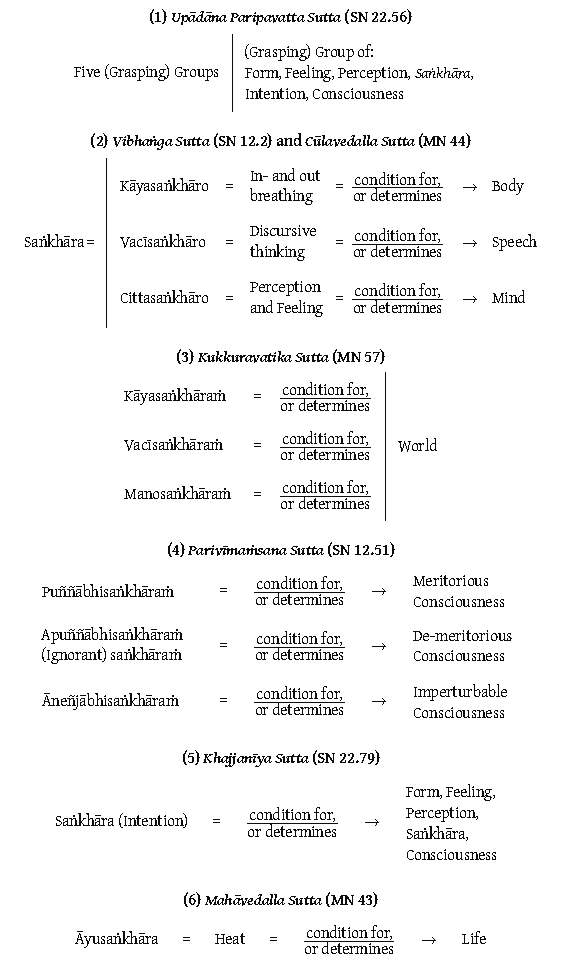
\includegraphics[width={\textwidth+10mm}]{./manuscript/tex/diagrams/sankhara-meanings.pdf}

\clearpage

\emph{Saṅkhāra}, therefore, in short means: a determination, or \authoremph{necessary condition}. This one meaning covers all uses of this word.

What is meant by determination or \authoremph{necessary condition} (that is to say, \emph{saṅkhāra}) must be distinctly understood. It means that whatever thing depends upon this necessary condition, that thing can exist \authoremph{only if} this necessary condition is present. The thing cannot be present without the necessary condition being present. If the necessary condition is absent, then the thing is also absent. It should not be understood as `once the necessary condition has come and gone the thing arises'. Nor must it be understood as `the necessary condition \authoremph{becomes} the thing'. No. There is no \authoremph{temporal} succession one after the other. If the necessary condition is gone, then the thing is also gone. This is a \authoremph{structural principle}.

It should also be clearly understood that \emph{saṅkhāra} do not refer to the things \emph{(dhammā)} for which they form necessary condition. The things that are determined or upbuilt with the \emph{saṅkhāra} as necessary condition are called \emph{saṅkhatā dhammā} (determined things). These \emph{saṅkhatā dhammā} are, however, \authoremph{of the nature of saṅkhāra}. That is to say, these determined things in turn act as the necessary condition for other determined things.

For example, the Six Bases are necessary condition for Contact. This means that Contact cannot come about without the presence of the Six Bases. Thus, in this instance, the Six Bases are \emph{saṅkhāra} and Contact is a \emph{saṅkhatā dhammā}. But again, Contact which is on the one hand a \emph{saṅkhatā dhammā} is the necessary condition for something else, viz., Feeling. Without Contact, no Feeling. Thus Contact as a \emph{saṅkhatā dhammā} is also a \emph{saṅkhāra}, dependent upon which stands Feeling.

The same applies to the Five Grasping Groups. The Five Grasping Groups are \emph{saṅkhatā dhammā} with \emph{saṅkhāra} (primarily, intention) as necessary condition. But they are also the necessary condition for something else, viz., Grasping. Thus, the Five Grasping Groups are both \emph{saṅkhatā dhammā} and \emph{saṅkhāra}. That is what is meant by saying that all \emph{saṅkhatā dhammā} are in the nature of \emph{saṅkhāra}.

These implications of the word \emph{saṅkhāra}, have to be clearly understood. Quite a lot of the fanciful interpretations of the Buddha-word are due to not understanding the precise meaning of the word \emph{saṅkhāra} and the manner in which it is used in the Suttas.
